\section{Experiment}
\label{sec:methods}

%% Introduction
Because the Koopman model is linear, it can be used to design linear controllers for nonlinear dynamical systems.


%% Description of system
\subsection{Description of System: Soft Arm with Laser Pointer}

The soft robot system used in experiments consists of two sections composed of three pneumatically driven McKibben actuators (also known as Pneumatic Artificial muscles or PAMs) adhered to a central foam spine by latex rubber suspended from a raised platform (see Fig. \Dan{Add figure with photo and schematic of robot}) .
The PAMs in the upper and lower sections are internally connected and arranged such that they share three input pressure lines and for any bending of the upper section, there is bending in the opposite direction in the bottom section.
This ensures that the laser pointer mounted to the end effector roughly points down at all times.
Roughly 30 cm beneath the hanging arm lies a flat board where the laser dot is projected.
A digital webcam aimed at the board is used to capture the position of the laser dot during trials.

%% Rig figure
\begin{figure}
    \centering
    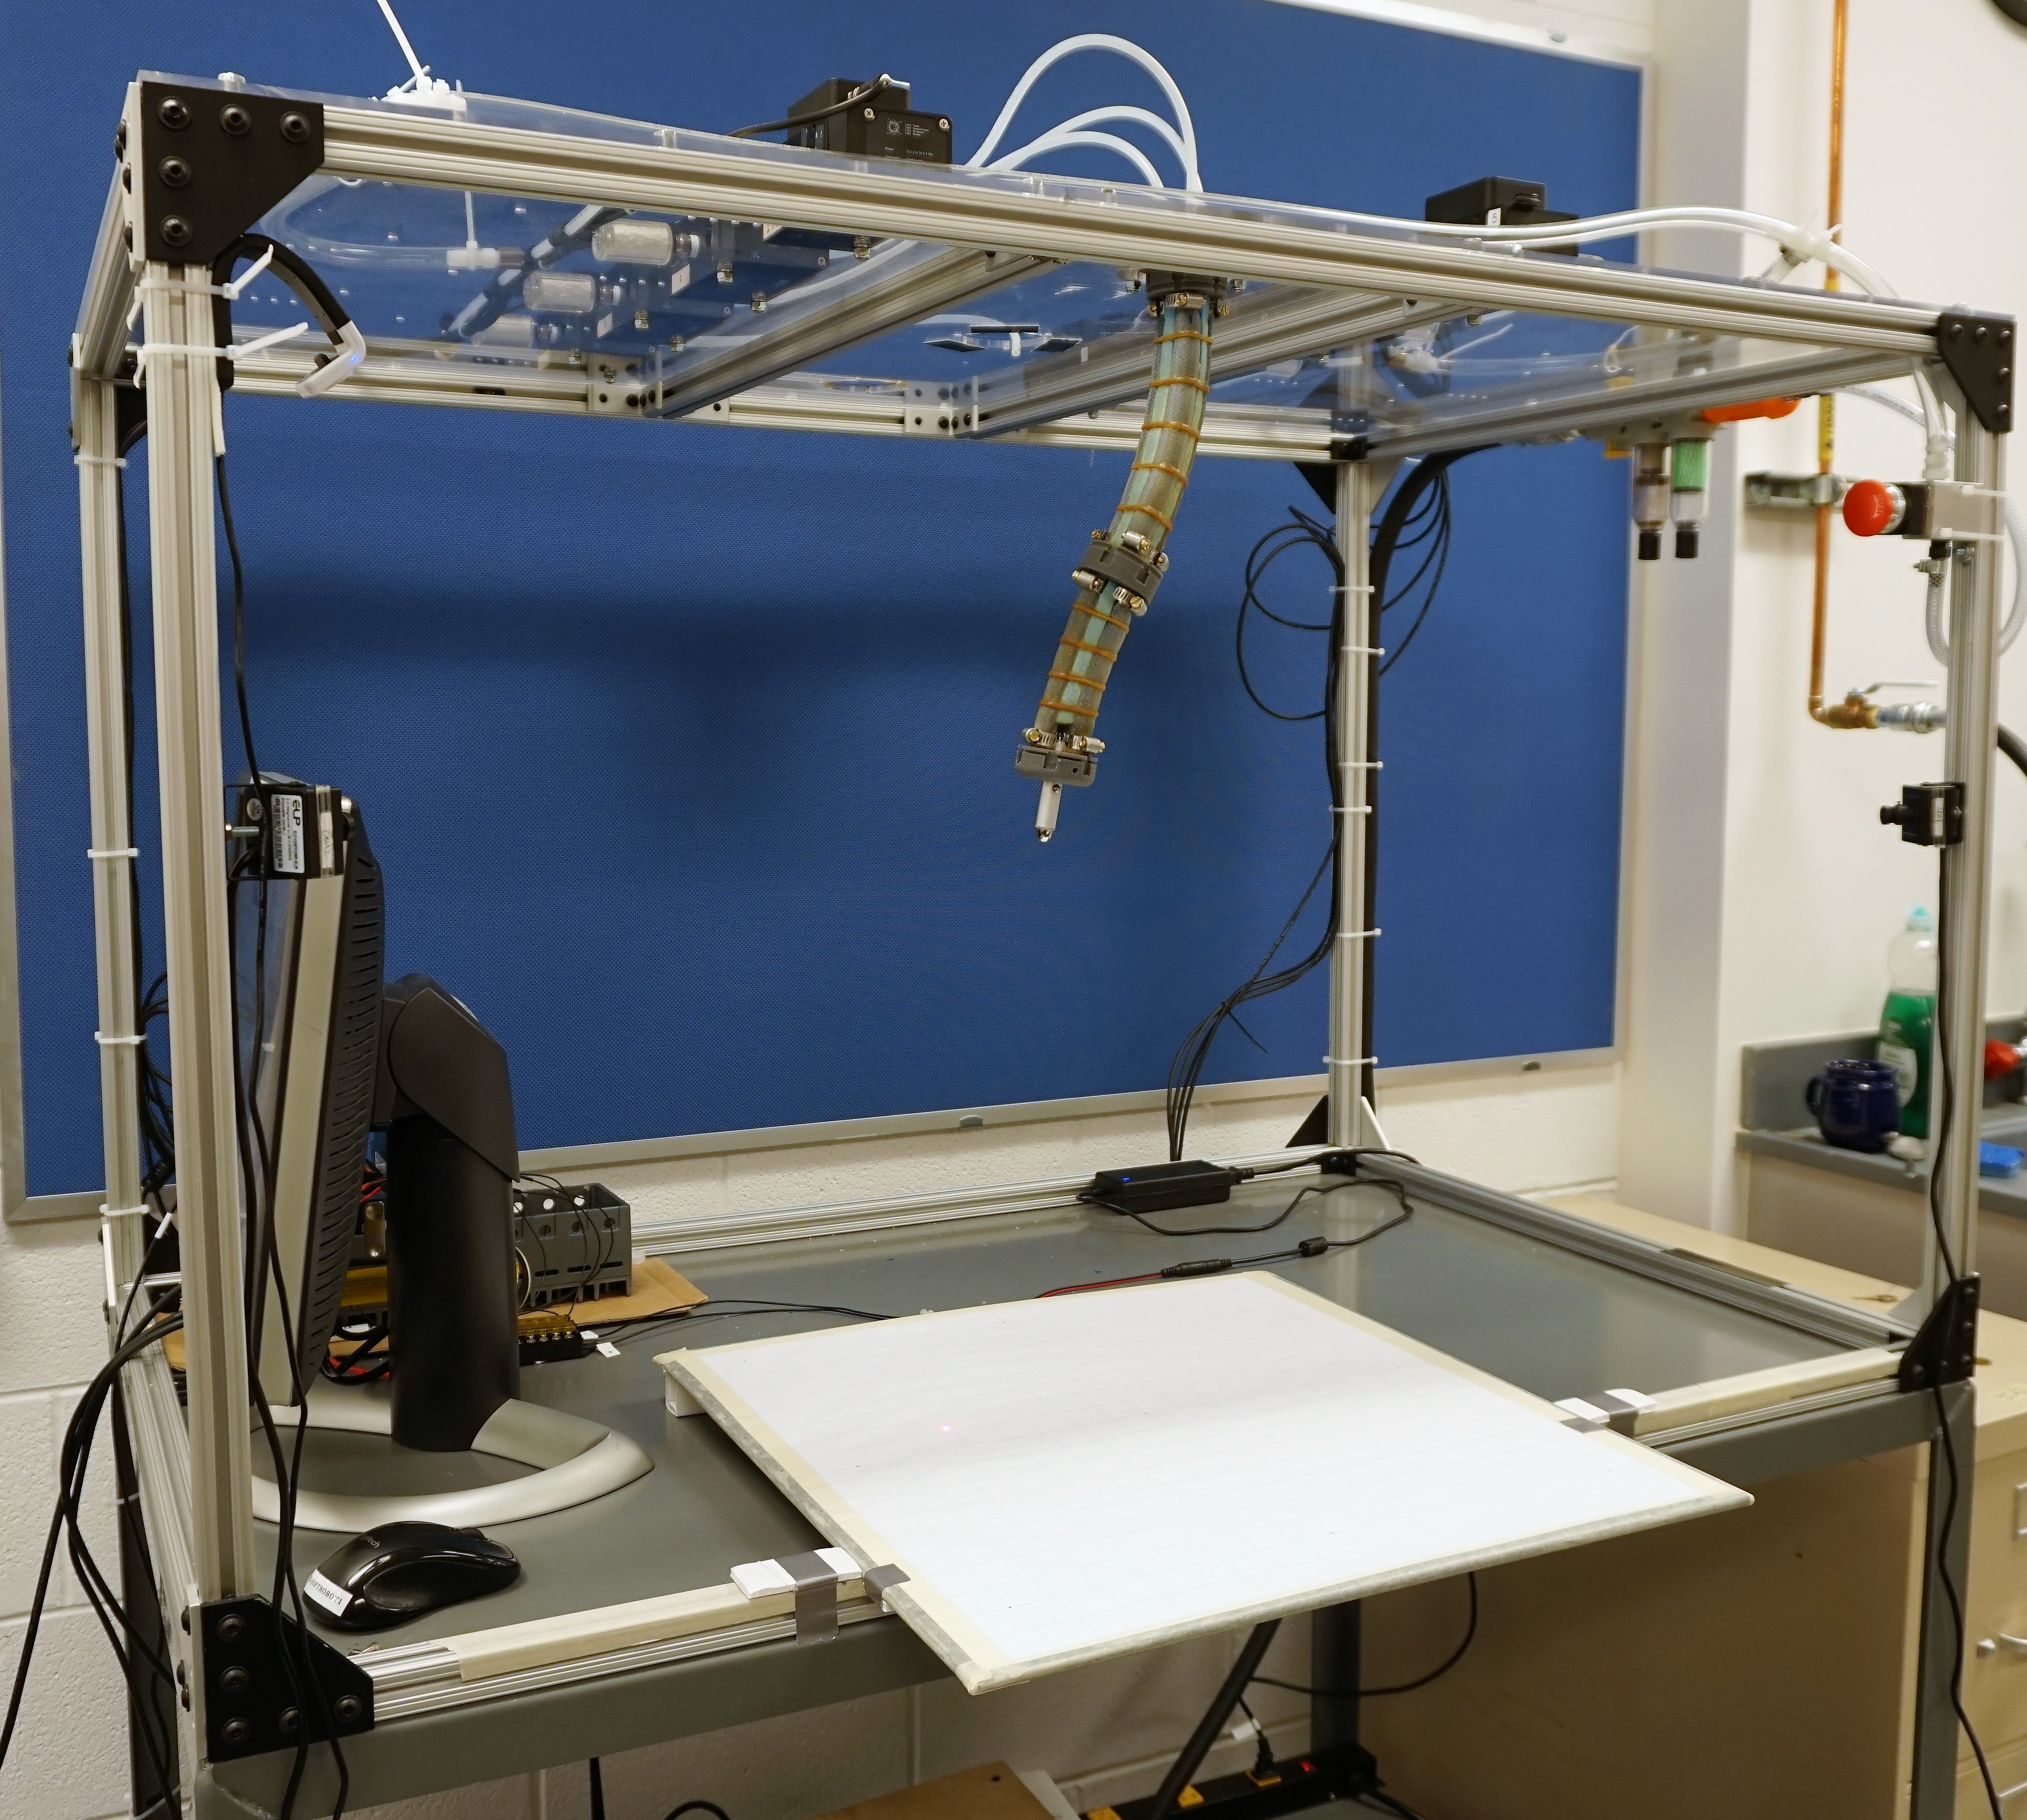
\includegraphics[width=\linewidth]{figures/DSC00707_cropped.jpg}
    \caption{\Dan{current placeholder for version with labels and possibly with background photoshopped out.}}
    \label{fig:rig}
\end{figure}

%% Robot figure
\begin{figure}
    \centering
    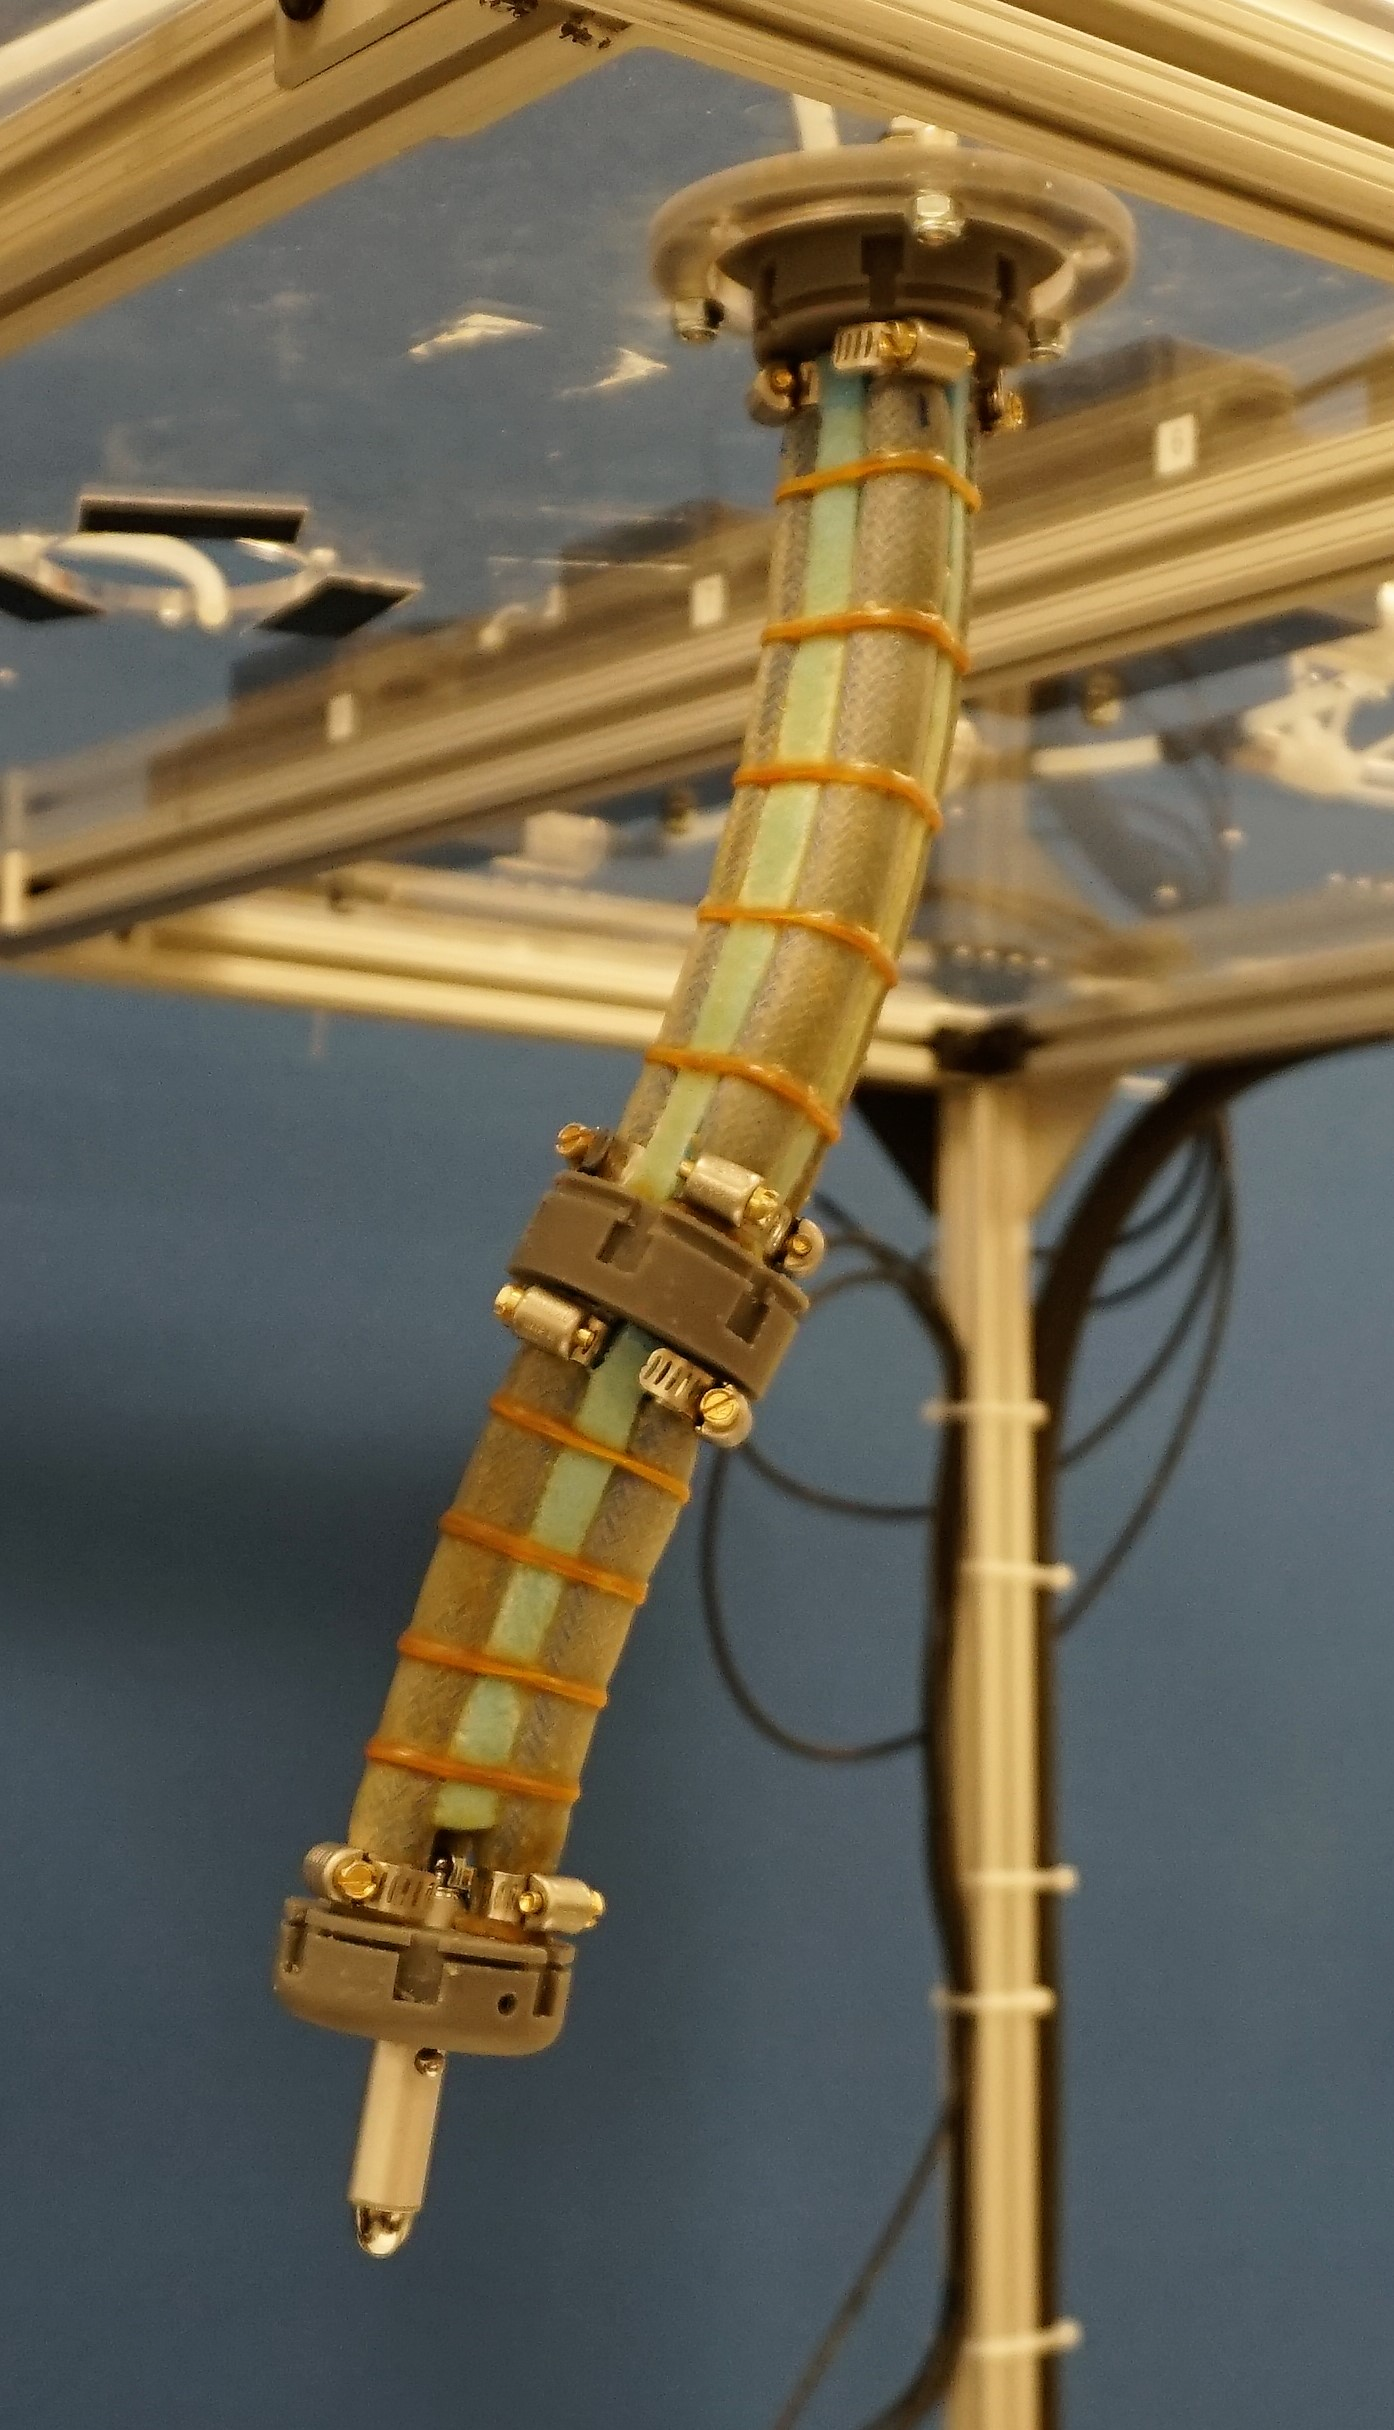
\includegraphics[width=0.5\linewidth]{figures/closeup.jpg}
    \caption{\Dan{Will also include a closeup of robot like this if space permits}}
    \label{fig:robot}
\end{figure}

%% Description of compared controllers
\subsection{Description of Controllers}

\begin{itemize}
    \item K-MPC: Koopman model predictor
    \item L-MPC: linear state-space model predictor
    \item N-MPC: nonlinear neural network model predictor
\end{itemize}

\subsubsection{Linear MPC}

%% Linear MPC optimization problem
\begin{equation}
\begin{aligned}
& \underset{u_{i} , x_{i}}{\text{min}}
& & z_{N_p}^{T} P z_{N_p} + \cdots \\
&&& \cdots + \sum_{i=0}^{N_p - 1} z_i^T Q z_i + u_i^T R u_i + q^T z_i + r^T u_i\\
& \text{s.t.}
& & z_{i+1} = A z_i + B u_i , \; i = 0 , \ldots , N_p - 1 \\
&&& E z_i + F u_i \leq b , \; i = 0 , \ldots , N_p - 1 \\
&&& z_0 = \psi(x_k).
\end{aligned}
\end{equation}


\subsubsection{Nonlinear MPC}

%% Nonlinear MPC optimization problem
\begin{equation}
\begin{aligned}
& \underset{u_{i} , x_{i}}{\text{min}}
& & z_{N_p}^{T} P z_{N_p} + \sum_{i=0}^{N_p - 1} z_i^T Q z_i + u_i^T R u_i + q^T z_i + r^T u_i\\
& \text{s.t.}
& & z_{i+1} = f( z_i , u_i ) , \; i = 0 , \ldots , N_p - 1 \\
&&& E z_i + F u_i \leq b , \; i = 0 , \ldots , N_p - 1 \\
&&& z_0 = \psi(x_k).
\end{aligned}
\end{equation}

%% Description of task
\subsection{Description of Task}

The performance of the various controllers was assessed with respect to a set of three trajectory following tasks.
Each task was to follow a reference trajectory as it traced out the following shapes:
\begin{enumerate}
    \item Block letter M (see Fig. \ref{fig:compare_blockM})
    \item Pacman (see Fig. \ref{fig:compare_pacman})
    \item TBD.
\end{enumerate}
The error for each trial was quantified as the root-mean-square error (RMSE) at each time step over the length of the trial.
The RMSE error for each controller and trial is presented in Table \ref{tab:RMSE}.